% Teilauswertung 2

\newpage
\section{Konzentrationsabhängigkeit von Schichtdicken}
\label{sec:konzDicke}
Zuerste werden die ermittelten Schichtdicken gegen die Polymerkonzentration aufgetragen:

\begin{center}
	\captionsetup{type=figure}
	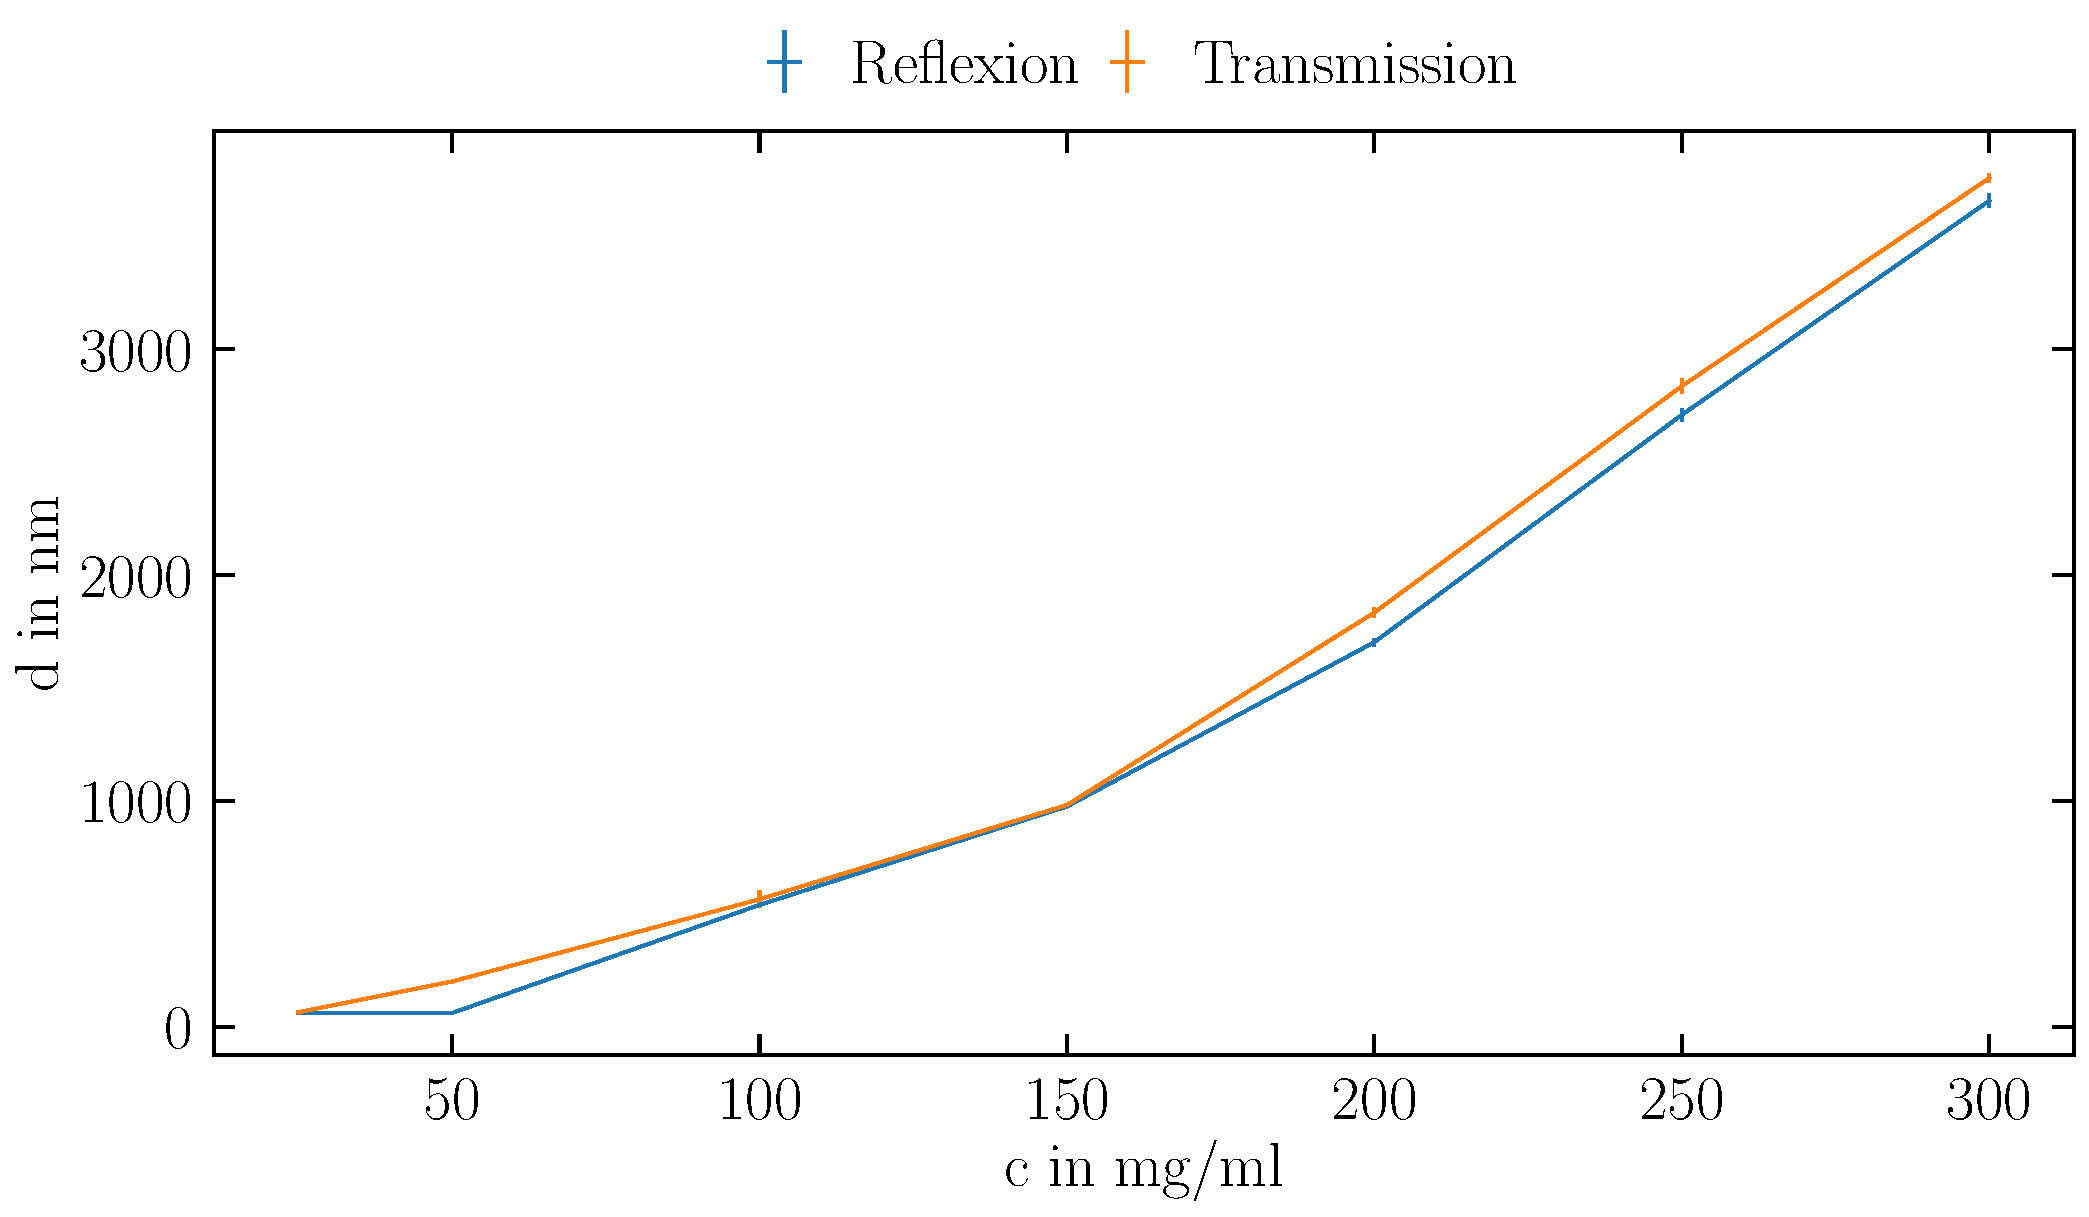
\includegraphics[width=0.92\textwidth]{Auswertung/43/Schichtdicken-Beide.pdf}
	\captionof{figure}{Schichtdicken $d$ der Proben in Abhänigkeit von der Konzentration der Polymerlösung $c$.}
	\label{fig:fitgueteReflexion}
\end{center}

Besoders hervorstechend ist ein Knickpunkt bei etwas über $150$ mg/ml rechts von disem scheint eine lineare Abhängikeit zwischen Konzentration und Schichdicke zu bestehen.

Links von dem Knickpunkt ist auch eine lineare abhänigkeit vorstellbar, jedoch fällt für niedrige Konzenrationen auf, dass mochlicherweise eine asymtotische Annäherung gegen eine Minimaldike stattfindet. Dies wird besonders deutlich wenn die durch Reflexion gewonnenen Messwerte betrachtet werden. Wohingegen eine linearer Abfall bei den Messwerten der Transmission vermutet werden kann. Prinzipiell würde eine Annäherung zu einer Minimaldicke plausibel wirken, da man vermuten könnte, dass sich eine Polymer-Monolage für kleine Konzentrationen ausbildet. Auch die Größenordnung, von um die $60$ nm, dieser kleinsten Dicke setzt dem nichts entgegen.

Abgesehen von den Differenzen bei kleinen Konzentrationen ist noch eine kleine Verschiebung bei großen Konzentrationen zu sehen. Jedoch scheint diese vernachlässigbar zu sein.


\newpage
\subsection{Bestimmung der kritischen Überlapp-Konzentration $c_0$}

Zur Bestimmung der kritischen Überlapp-Konzentration wurde im Bereich vor und nach dem Knick je ein linearer Fit durchgeführt. Somit konnte die Stelle des knicks und die kritischen Überlapp-Konzentration genau bestimmt werden.

Verwendete Fitfunktion:
\begin{gather}
	y = ax + b
	%\caption[]{Lineare Fitfunktion}
\end{gather}

Fit:
\begin{center}
	\captionsetup{type=figure}
	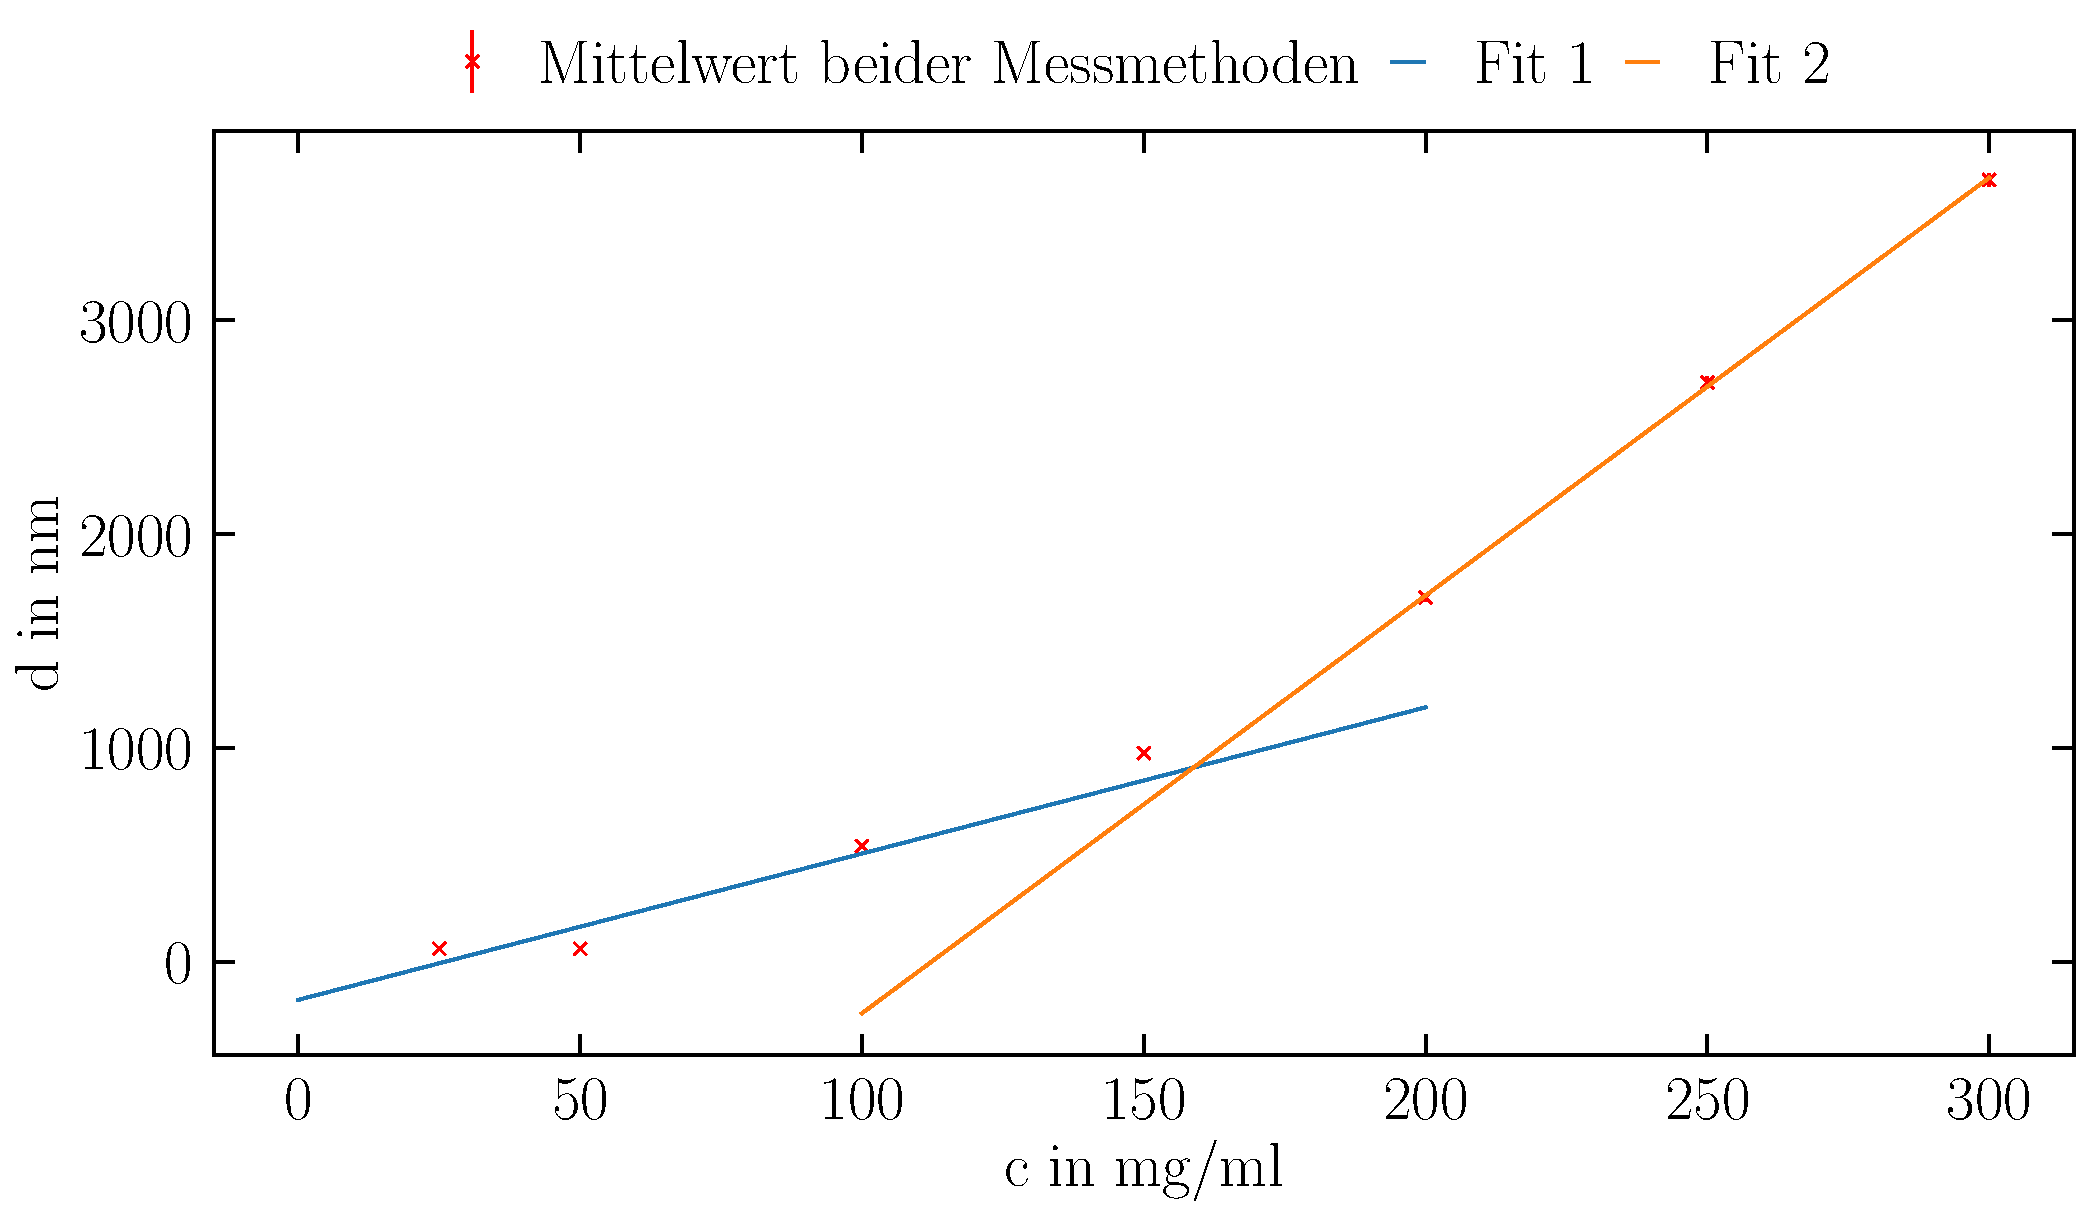
\includegraphics[width=0.92\textwidth]{Auswertung/43/Schichtdicken-Fit.pdf}
	\captionof{figure}{Mittelwert der Schichtdicken $d$ der Proben, aus beiden Messwerten, in Abhänigkeit von der Konzentration der Polymerlösung $c$. Und lineare Fits zur ermittelung der kritischen Überlapp-Konzentration $c_0$.}
	\label{fig:fitgueteReflexion}
\end{center}

\begin{table}[h]
	\centering
	\begin{tabular}{r|c|c}
		& a & b \\ \hline
		Fit 1 & 6,84 & -178,86 \\
		Fit 2 & 19,54 & -2195,79
	\end{tabular}
	\caption[]{Ergebnisse des linearen Fits.}
\end{table}

Da $c_0$ die x-Koordinate des Schnittpunktes ist, kann die volgendermaßen berechnet werden:
\begin{align}
	c_0 &= \frac{b_2 - b_1}{a_1 - a_2}\\
	\Rightarrow c_0 &= (159 \pm 1) \, \frac{\text{mg}}{\text{ml}}
\end{align}

\subsection{Berechnung der root-mean-square end-to-end distance}

\paragraph*{Nach Mark}
Die root-mean-square end-to-end distance wird im folgenden, ausgehend vom charakteristischen Flory Verhältnis von $C_\infty = 9.5$ berechnet. Heirzu wird folgende Formel benutzt:
\begin{gather}
	R_{rms} = \sqrt{C_\infty n l^2}
\end{gather}
Wobei $l$ die Länge im Polymerrückrat ist (Annahme: $l = 1.54$ Anström) und n die Anzahl der Bindungen im Polymerrückrat ist. (??)

\paragraph*{Nach Daum}
Nun wird root-mean-square end-to-end distance mittels folgender Formel berechnet:
\begin{gather}
	R_{rms} = 2,84 \cdot 10^{-8} \cdot \sqrt[3]{\frac{M}{c_0}}
\end{gather}
Wobei $M$ das Molekulargewicht des Polymers ist und $c_0$ die kritische Überlapp-Konzentration.

\subsection{Vergleich der Messdaten mit den bekannten Polymer Modellen}